%todo titel!!
\chapter{Fachbezogene Grundlagen} \label{sec:fachgrund}
Zunächst sollen die Entwicklungsumgebung und die aktuelle Implementation in der Software näher betrachtet werden. Im Anschluss wird noch das erarbeitete Konzept des \ac{fra} vorgestellt.

%situation auf der Kamera etc
\section{Kontext}
Um einen Überblick über das Umfeld der Arbeit zu bekommen, werden ein paar Grundlagen und auch die Funktionsweise einer Kamera betrachtet. 

\subsection{Kamera}
Um die Funktionalität des \ac{fra} festzustellen und grobe Fehler rechtzeitig zu erkennen, ist das regelmäßige Testen auf der Zielplattform unerlässlich. 
Die Wahl der Kamera ist auf eine \ac{ARRI} AMIRA gefallen, da die Entwicklungsumgebung durch vorherige Arbeit bekannt ist. Zusätzlich ist sie nicht die aktuellste Kamera der Firma \ac{ARRI} und somit ohne Probleme verfügbar.

%https://www.arri.com/resource/blob/33916/909908b1643addb99036f132d6b3582c/amira-product-image-data.jpg
%todo footnote
\begin{figure}[!hbtp]
	\centering
	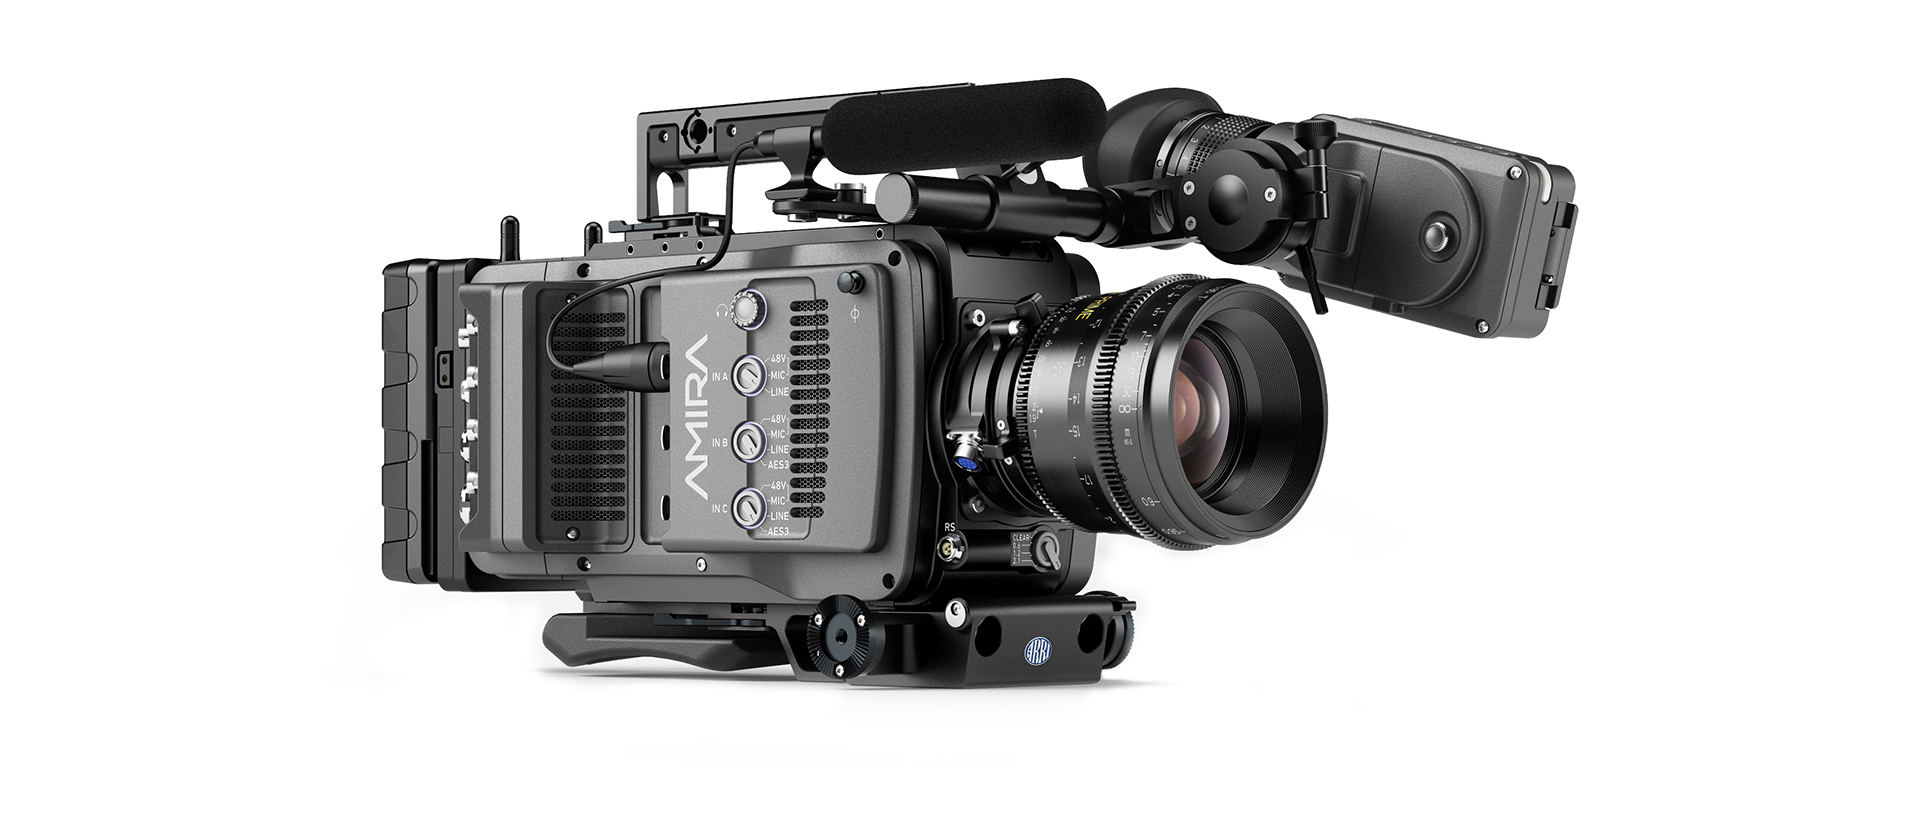
\includegraphics[width = 0.7\linewidth]{pictures/amira-product-image-data.jpg}
	\smallskip
	\caption{ARRI AMIRA \protect\footnotemark[2]}
	\label{fig:amira}
\end{figure}  
\footnotetext[2]{ \url{https://www.arri.com/resource/blob/33916/909908b1643addb99036f132d6b3582c/amira-product-image-data.jpg}}

Die AMIRA ist eine vielseitige Kamera, die für eine Einmannbedienung ausgelegt ist.
Zusätzlich ist sie mit einem Audioboard ausgestattet und aus diesem Grund bei Dokumentationsfilmen und der elektronischen Berichtserstattung gerne verwendet. Zum Beispiel wird die \ac{ARRI} AMIRA bei Sportveranstaltungen der NFL in Amerika eingesetzt. \cite{arrinewsamira} 

Für Spielfilm- und Serienproduktionen wird auch manchmal die \ac{ARRI} AMIRA eingesetzt, wodurch das breite Einsatzspektrum der Kamera noch deutlicher wird.
Als Beispiele sind hier der bayrische Eberhofer Krimi \glqq Sauerkrautkoma\grqq{} \cite{arrikrimi}, die Netflixserie \glqq The Ivory Game\grqq{} \cite{imdbivory} oder auch das Fernsehmagazin \glqq The Grand Tour\grqq{} \cite{imdbtour} zu nennen.

% Elektronische Berichtserstattung, billigste, neues marktsegement, keine andere arri kamera drinnen, live sendung bis hin zu reportage, viel bei broadcast unternehmen und sportveranstaltungen
%doku: the ivery game (netflix),  doku & aktion, super bild, und audiopoard, top gear (amazon), serien udn spielfilm (eberhofer filme), veep (us), sportveranstalungen (nfl nba) us, 2 bis 6 Kameras
%eb kamera, broadcaster, live sendung bis reportage

\subsection{Bildkette}
Unter einer Bildkette versteht man die Verarbeitungskette der Bilder vom Eingang - dem Sensorbild bis zu zum Ausgang, in unserem Fall die \ac{rec} und das \ac{sdi}.

\begin{figure}[!hbtp]
	\centering
	\includegraphics[width = \linewidth]{pictures/bildkette.png}
	\smallskip
	\caption{Schematische Bildkette}
	\label{fig:bild}
\end{figure} 

In der Abbildung~\ref{fig:bild} sieht man eine schematische Bildkette, die in dieser Arbeit zur Veranschaulichung weiter detailliert wird. 
Von der Quelle bis zur jeweiligen Senke läuft das Bild durch verschiedene Module, die für die Anpassung des Bilds sorgen. 

Direkt nach dem Sensor geht das Bild durch eine \acl{xbar}, hier wird das identische Bild in zwei Bildpfade weitergeführt. Für die \acl{rec} wird das Bild im Crop zugeschnitten, somit wird nur ein bestimmter Bildausschnitt aufgezeichnet. In dem anderen Bildpfad wird, mithilfe des Scalers, das Bild kleiner skaliert. Nachdem eine grafische Benutzeroberfläche hinzugefügt worden ist, wird das Bild am \ac{sdi} ausgegeben. Hier ist durch die Skalierung das komplette Sensorbild einschließlich der eingefügten Oberfläche zu sehen.

In dieser Arbeit wird nur das \ac{fpga}-Modul \ac{xbar} softwareseitig implementiert, da weitere Module sonst den Umfang der Arbeit überschreitet. 


\subsection{Funktionsweise}
Bevor auf das erarbeitete Konzept eingegangen wird, soll kurz auf die Funktionsweise der Kamera und die aktuelle Implementierung eingegangen werden.

Die bildverarbeitende Hauptfunktionalität liegt im \ac{fpga}. Hier werden die Module entsprechend der Bildkette angeordnet und verbunden. Durch die Software werden bei den \ac{fpga} Module Einstellungen vorgenommen.\\


Damit die Einstellungen auch zu dem Sensorbild passen, werden alle Module des \ac{fpga}s in dem \ac{geo} abgebildet. Das objektorientierte Framework führt hauptsächlich Berechnungen der Bildgrößen und Offsets durch. Nach der Änderung einer Größe in der Quelle oder Senke werden alle Module in der abgebildeten Frameworkbildkette geupdatet und entsprechend der voreingestellten Parameter werden die Größen neu berechnet. 

Nach der Änderung der Größen wird in dem entsprechenden Modul ein Flag gesetzt, welches später dafür sorgt, dass auch das Modul im \ac{fpga} aktualisiert wird. 

Beim Updaten des Modules wird an den entsprechenden Offset im \ac{fpga} die übergebenen Einstellungen geschrieben und gleichzeitig das gesetzte Flag wieder gelöscht. 

%todo umschreiben 
Damit der Zugriff auf den \ac{fpga} möglich ist, wird dieser beim Starten der Software über ein \ac{ioctl} initialisiert und anschließend kann über eine Variable im Shared Memory in allen Prozesseen darauf zugegriffen werden.

\subsection{Problematik}\label{sec:prob}
Bei der aktuellen Implementierung liegen verschiedene Probleme vor, die durch ein neues Framework eliminiert werden sollen.\\

Zum Einen muss bei den Zugriff auf ein Modul immer der \ac{fpga} gesperrt werden. Dadurch kann es passieren, dass es einen oder zwei Frames dauert, bis alle Einstellungen in der Bildkette aktuell sind.\\


Des weiteren müssen die Adressen für die \ac{fpga} Module händisch eingetragen werden. Die Fehleranfälligkeit steigt dadurch natürlich weiter, da es passieren kann, dass die Software, Einstellungen an eine Adresse schreibt, hinter der kein Modul liegt. In schlechtesten Fall werden die Register eines anderen Modules beschrieben und es kommt zum Fehlerfall in der Bildkette.\\


Auch die Länge der Register wird in der aktuellen Implementierung nicht weiter berücksichtigt. So kann es dann passieren, dass über ein Register hinweg geschrieben wird. Auch dann kommt es zum Fehlerfall in der Bildkette, da andere Einstellungen überschrieben werden. 
 
%v.4.15.9
\section{Konzept}\label{sec:konzept}
Die Probleme in der aktuellen Implementierung (siehe Kapitel~\ref{sec:prob}) sollen durch ein neues Framework behoben werden, aber die Zugriffe der Software auf den \ac{fpga} sollen auch übersichtlicher und wartbarer gestaltet werden. \\

Die Zugriffe auf den \ac{fpga} benötigen in der momentanen Implementierung immer die Adressen der Module im \ac{fpga}. Dadurch wird die Fehlersuche in diesen Teilen der Software extrem kompliziert und aufwendig. Durch das \ac{fra} sollen die Firmware Module im Kernel als Gerät angelegt werden und in der Software wird auf die \ac{fpga} Module über die entsprechenden Dateideskriptoren zugegriffen. \\


Die Geräte werden mit der Adresse, dem Name, dem Type und der Größe des dahinterstehenden Modul angelegt. Dieser Teil soll generisch generiert werden, aber aufgrund von verschiedenen Abhängigkeiten überschreitet es den Umfang der Arbeit. Deswegen werden die Geräte beim Initialisieren des Bildpfads mit den entsprechenden Parametern angelegt. \\

Das Öffnen der Dateideskriptoren erfolgt in der Software über den Namen und wird in einem Handle gespeichert. Damit ist der Zugriff ohne Adresse gewährleistet. Jeder Prozess in der Software muss seinen eigenen Dateideskriptor öffnen und verwaltet somit ein eigenes Handle. 
Im Kernel wird gewährleistet, dass nur eine maximale Anzahl von Deskriptoren geöffnet werden kann. Zusätzlich soll implementiert werden, dass es verschiedene Applikationstypen gibt. Damit kann immer nur eine echte Applikation Zugriff bekommen, allerdings sollen Debugtools immer die Möglichkeit haben zu lesen und teilweise auch zusätzlich Schreibrechte. \\

Der Zugriff auf die Module erfolgt über ein \ac{ioctl} des Treibers. Da beim Anlegen der Geräte eine Größe festgelegt wird, soll bei allen Zugriffen auf die Register überprüft werden, ob diese innerhalb der angegebenen Modulgröße liegen. Damit ist es nicht mehr möglich über ein Register hinweg zu schreiben.\\



